\documentclass[12pt]{article}

%useful packages
\usepackage{color,soul}
\usepackage[usenames,dvipsnames,svgnames,table]{xcolor}
\usepackage{amsmath,amsthm,amscd,amssymb,bm}
\usepackage{hyperref}
\hypersetup{
    colorlinks=true,
    linkcolor=JungleGreen,
    urlcolor  =JungleGreen,
    citecolor = JungleGreen,
    anchorcolor = JungleGreen
}
\usepackage[utf8]{inputenc}
\usepackage[top=2cm, bottom=3cm, left=2cm, right=2cm]{geometry}
\usepackage{pgfplots}
\usepackage{enumitem}
\usepgfplotslibrary{fillbetween}
\usetikzlibrary{patterns}
\usepackage{tcolorbox}
\usepackage{centernot}
\usepackage{mathtools}
\usepackage{xcolor}
\usepackage{subcaption}

%personal definitions and commands
\newcommand{\R}{\mathbb{R}} 
\newcommand{\E}{\mathbb{E}}
\newcommand{\V}{\mathbb{V}}
\newcommand{\C}{\mathbb{C}}
\newcommand{\Prob}{\mathbb{P}}
\newcommand{\e}{\epsilon}
\newcommand\numberthis{\addtocounter{equation}{1}\tag{\theequation}} %allows numbering of single equations in align* environment
\newcommand{\mtx}[1]{\ensuremath{\bm{\mathit{#1}}}}
\newcommand{\B}{\hat{\boldsymbol{\beta}}}
\newcommand{\Cov}{\mathbb{C}\text{ov}}
\newcommand{\N}{\mathcal{N}}



\title{ECON641 -- Problem Set 2}
\author{Anirudh Yadav}
\setlength\parindent{0pt}
\begin{document}

\maketitle

\setcounter{tocdepth}{2}
\tableofcontents

\newpage

\section{The Firm Size Distribution}

\subsection{Power law in firm size}
A random variable $S$ follows a power law if
\begin{align}
\Pr[S>s] &= Cs^{-\zeta}, \text{ with } C, s>0 \label{eq:pl1}\\
\implies \log \Pr[S>s] &= \log C- \zeta s. \nonumber
\end{align}
Note that Zipf's law refers to a power law distribution with exponent $\zeta \approx 1$. Recent research has shown that the distribution of firm size is approximately described by Zipf's law. Below, we're going to explore the application of these ideas to Compustat data.\\

Before I get into the data work, let's briefly try to understand why we're doing all of this log-rank/log-size stuff. Suppose $S$ follows a power law as in (\ref{eq:pl1}). Then, draw $N$ realizations and rank them in descending order $S_{(1)} > S_{(2)} > ... > S_{N}$. Because of the ranking, we get $i/N = 1- F(S_{(i)})$ (since $F(S_{(i)})$ is distributed standard uniform). Thus, $i/N = CS_{(i)}^{-\zeta}$, or
\begin{align*}
\text{Rank}& = NCS_{(i)}^{-\zeta}\\
\implies \log \text{Rank} &= \text{constant} - \zeta \log S_{(i)}.
\end{align*}

\subsubsection{Firm sales}
First, I plot the log--log plot of rank vs. sales for all firms in the Compustat database for 2015. Clearly, the relationship is not linear, suggesting that the firm size distribution does not follow a power law. This result is consistent with Stanley, \textit{et. al.} (1995), who also use Compustat data. Note that Axtell (2001) uses US Census data (which obviously contains a far more comprehensive sample of firms compared to Compustat) and finds that the firm size distribution does indeed follow Zipf's law.

\begin{figure}[htbp!]
\centering
\caption{\textbf{Sales Distribution of All Firms in Compustat in 2015}}
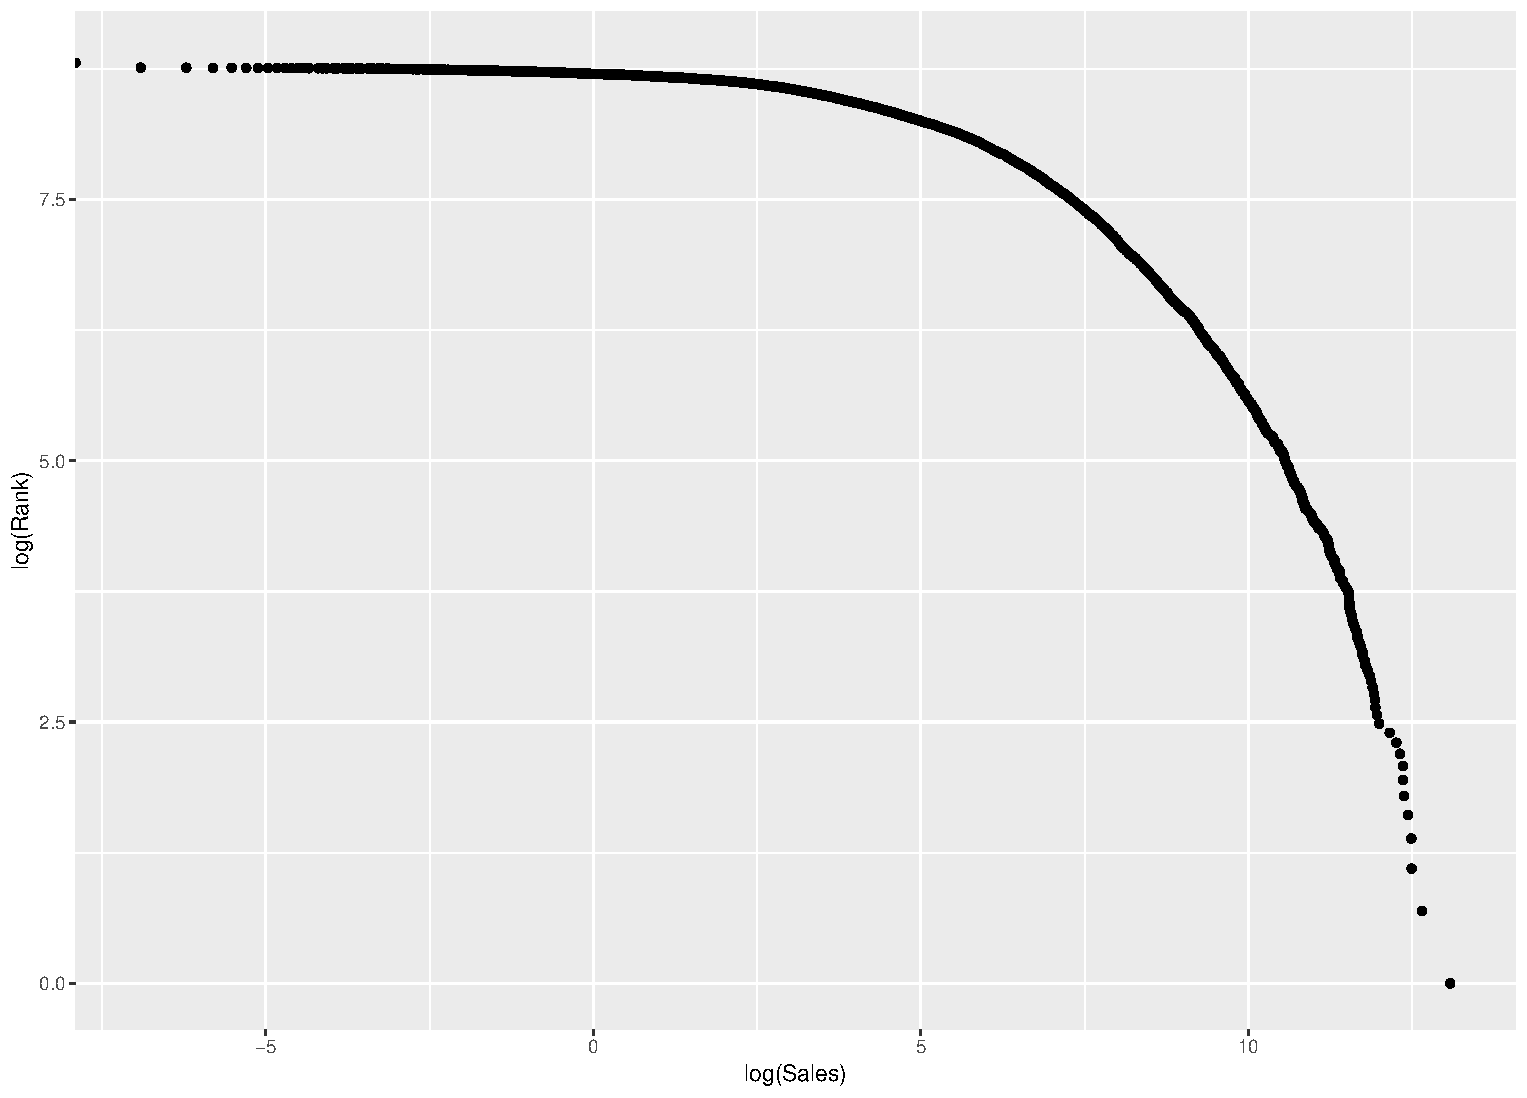
\includegraphics[width=0.55\textwidth]{2015-sales-full.pdf}
\label{fig1}
\end{figure}

Next, I plot the log--log sales plots for the top 500 and 100 firms in the Compustat database. In both cases, there seems to be a linear relationship, suggesting that the tail of the firm sales distribution follows a power law.

\begin{figure}[htpb!]
    \centering
    \caption{\textbf{Sales Distribution for Top 500 and Top 100 Firms in 2015}}
    \begin{minipage}{0.5\textwidth}
        %\centering
        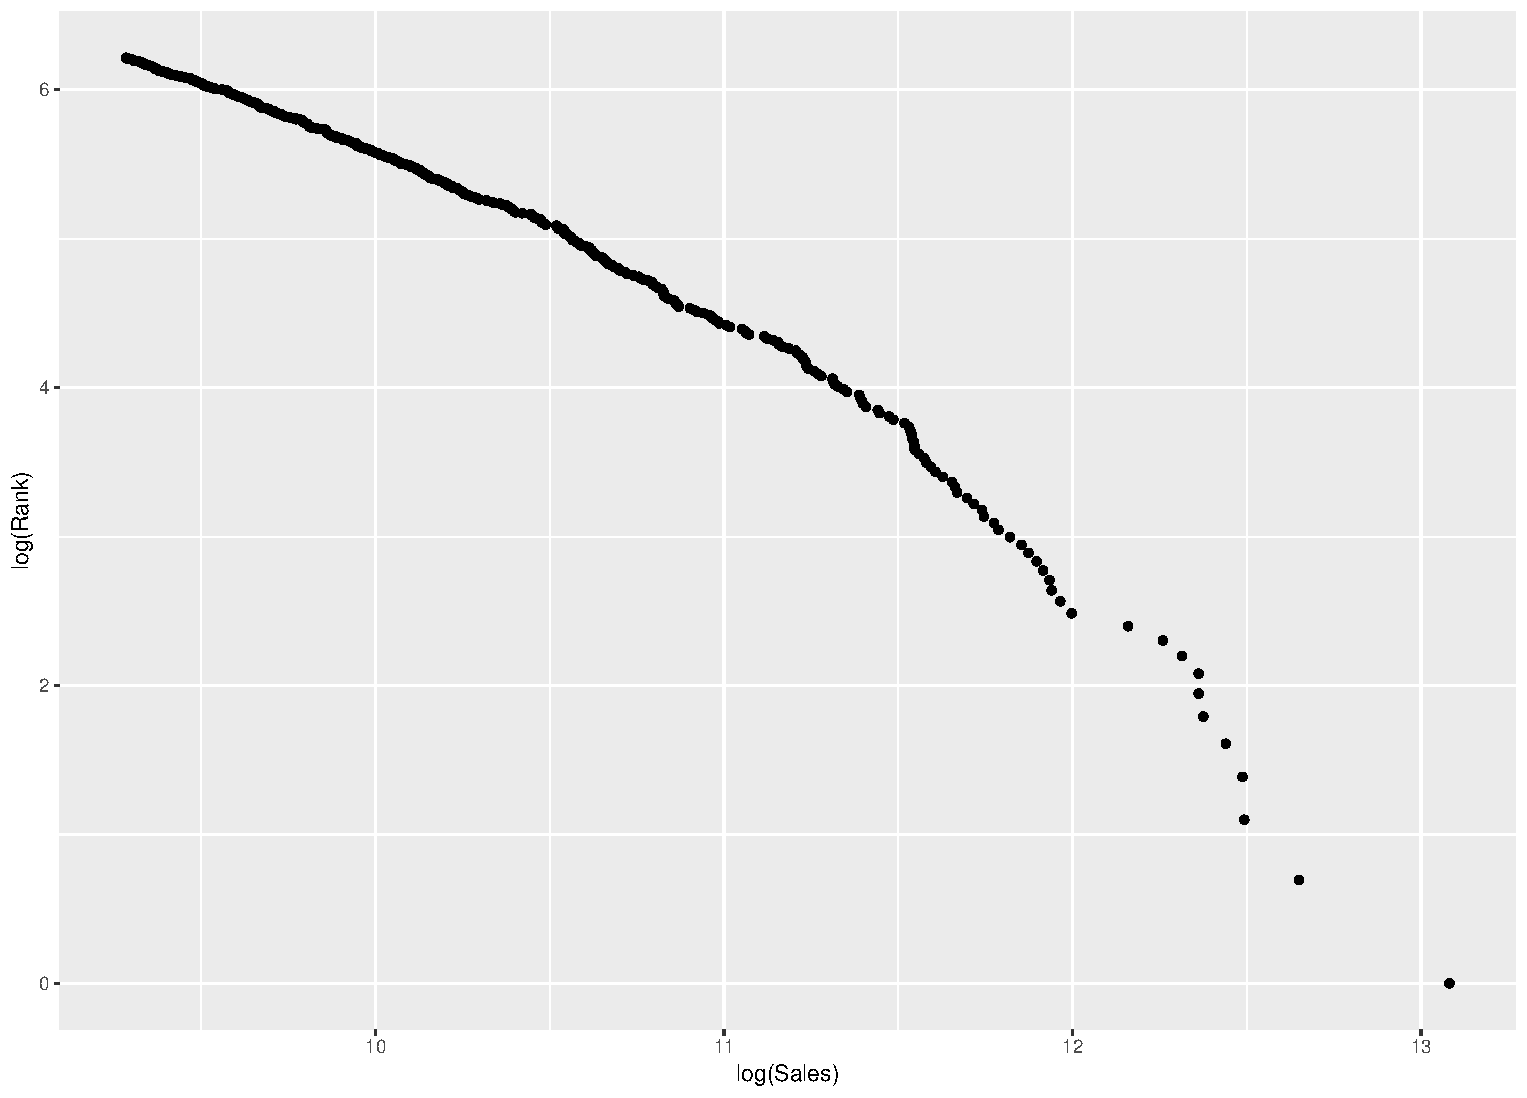
\includegraphics[width=1\textwidth]{2015-sales-500.pdf}
        \subcaption{Top 500 firms}
    \end{minipage}\hfill
    \begin{minipage}{0.5\textwidth}
      %  \centering
        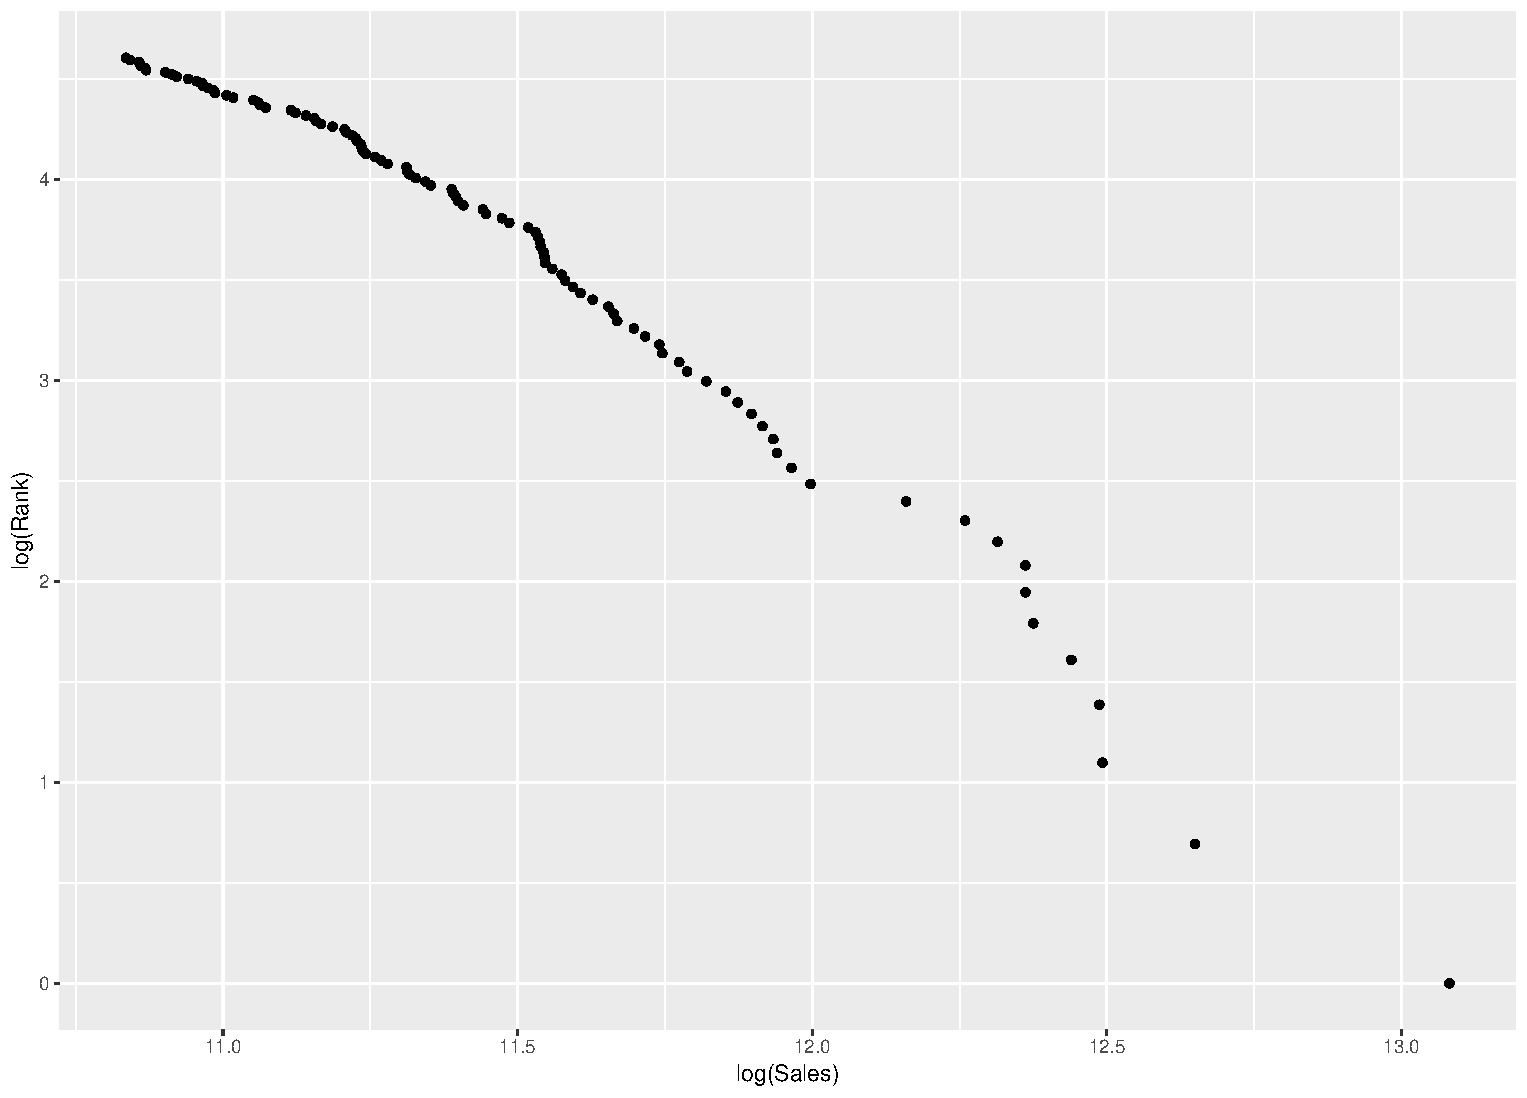
\includegraphics[width=1\textwidth]{2015-sales-100.pdf}
        \subcaption{Top 100 firms}
    \end{minipage}
\end{figure}

Next, I estimate the power law coefficient $\zeta$ using the estimator proposed by Gabaix and Ibragimov (2011) for the samples of firms above. That is, I estimate the model
\begin{align*}
\log(\text{Rank}_i - 1/2) = \text{constant} - \zeta \log S_{i} + \e_i
\end{align*}
using OLS. I compute standard errors as in Gabaix and Ibragimov (2011). Table 1 shows the estimation results -- suggesting that the sales distribution of the top 500 firms is approximately follows Zipf's law.

\begin{table}[htpb!]
\centering
\caption{\textbf{Estimated Power Law Coefficients for Firm Sales in 2015}}
For different lower size cutoffs\\
\begin{tabular}{lrrr}
  \hline
 & All firms & Top 500 & Top 100 \\ 
  \hline
$\hat{\zeta}$ & -0.27 & -1.28 & -2.06 \\ 
  Std. err. & 0.00 & 0.08 & 0.29 \\ 
   \hline
\end{tabular}
\end{table}

\subsubsection{Firm sales by industry}

\subsubsection{Employment}

\subsubsection{Employment by industry}

\subsubsection{Robustness check: 1985 data}





\end{document}
